\chapter{Resultados}

Foram realizados vários testes para encontrar o melhor modelo(rede) que atendessem os objetivos desta pesquisa, e após todo esse processo inicial, foi possível encontrar e definir os parâmetros da estrutura da RNA conforme a Figura 1.

Como mostra a Figura 1, a rede apresenta a configuração de 410 entradas, pois, as entradas foram restringidas a uma duração de 0,1 segundos, e a uma taxa de amostragem de 4096Hz, o que é mais do que suficiente para caracterizar os eventos usados nesta pesquisa, dado que os fenômenos cosmológicos considerados geralmente acontecem em menos de 0,1 segundos.

Durante o processo de testes a configuração que obteve o melhor resultado foi com uma camada oculta contendo 10 neurônios. A quantidade pequena de neurônios foi suficiente para conseguir a generalização máxima, para o problema da pesquisa. Notou-se que durante o processo de testes o aumento da quantidade de neurônios na camada oculta prolongava o treinamento e até certo a quantidade de neurônios não influenciava na generalização da RNA. Para manter uma RNA de baixo custo computacional optou-se pela menor quantidade de neurônios sem perda de generalização do processo, o que resultou em uma RNA extremamente leve em comparação a redes neurais profundas. 

A camada de saída se manteve constante com 2 neurônios, devido ao método adotado na pesquisa, que utilizou da equação~\ref{eq:score} para aprimorar a discriminação do resultado da RNA. Isto possibilitou a geração de duas distribuições do \textit{score}, uma para os classificados como Onda e uma para os classificados como Ruído.

E quanto aos parâmetros de treinamento o número máximo de iterações permaneceu o mesmo durante toda a pesquisa com 100000 iterações, apesar de que, em nenhum momento a rede atingiu esse limite, mesmo assim foi usado como critério de parada. O valor inicial para a taxa de aprendizado foi de 0,025 mas foi usado uma taxa adaptativa. A função de ativação na camada oculta foi a Logarítmica Sigmoide, a qual, é comumente utilizada por redes neurais com propagação positiva (Feedforward) que precisam ter como saída apenas números positivos, em redes neurais multicamadas. A função de ativação usada na camada de saída foi a Linear, pois, apresentou melhor resultado dado que esta função não altera a saída do neurônio. Em consequência do uso da equação~\ref{eq:score}  a função de ativação Softmax não foi cogitada, apesar de ser comumente usada em redes neurais de classificação.

Foi definido desde o inicio que a RNA usaria o algorítimo Backpropagation. Tendo em vista que, o algoritmo Levenberg-Marquardt~\cite{levenberg1944method} é uma combinação do algoritmo de descida de gradiente (Backpropagation) e o método de Gauss-Newton~\cite{bjorck1996numerical} com uma equação um pouco mais complicada, este algoritmo apresenta excelentes resultados. Graças a este algoritmo a rede apresentou uma acurácia melhor, mesmo que na fase de treinamento o tempo tenha dobrado, mas devido a simplicidade da rede o tempo de treinamento foi irrelevante.

Tanto o MSE quanto o KS foram utilizados como critério para definir a acurácia da rede, pois quanto menor o MSE melhor o resultado da RNA. Neste sentido a rede que apresentou o menor erro (MSE) possível, obtendo somente 0.000140842 de erro em apenas 5612 épocas de treinamento.

Consequentemente a RNA apresentou uma excelente discriminação das classe Onda e Ruído. A Figura~\ref{fig:histograma} mostra a distribuição do score gerado pela RNA, em que, a classe Onda tem uma distribuição do score centrada em torno de $1$, enquanto a classe Ruído tem uma distribuição do score em torno de $0$. 

\begin{figure}[H]
\centering
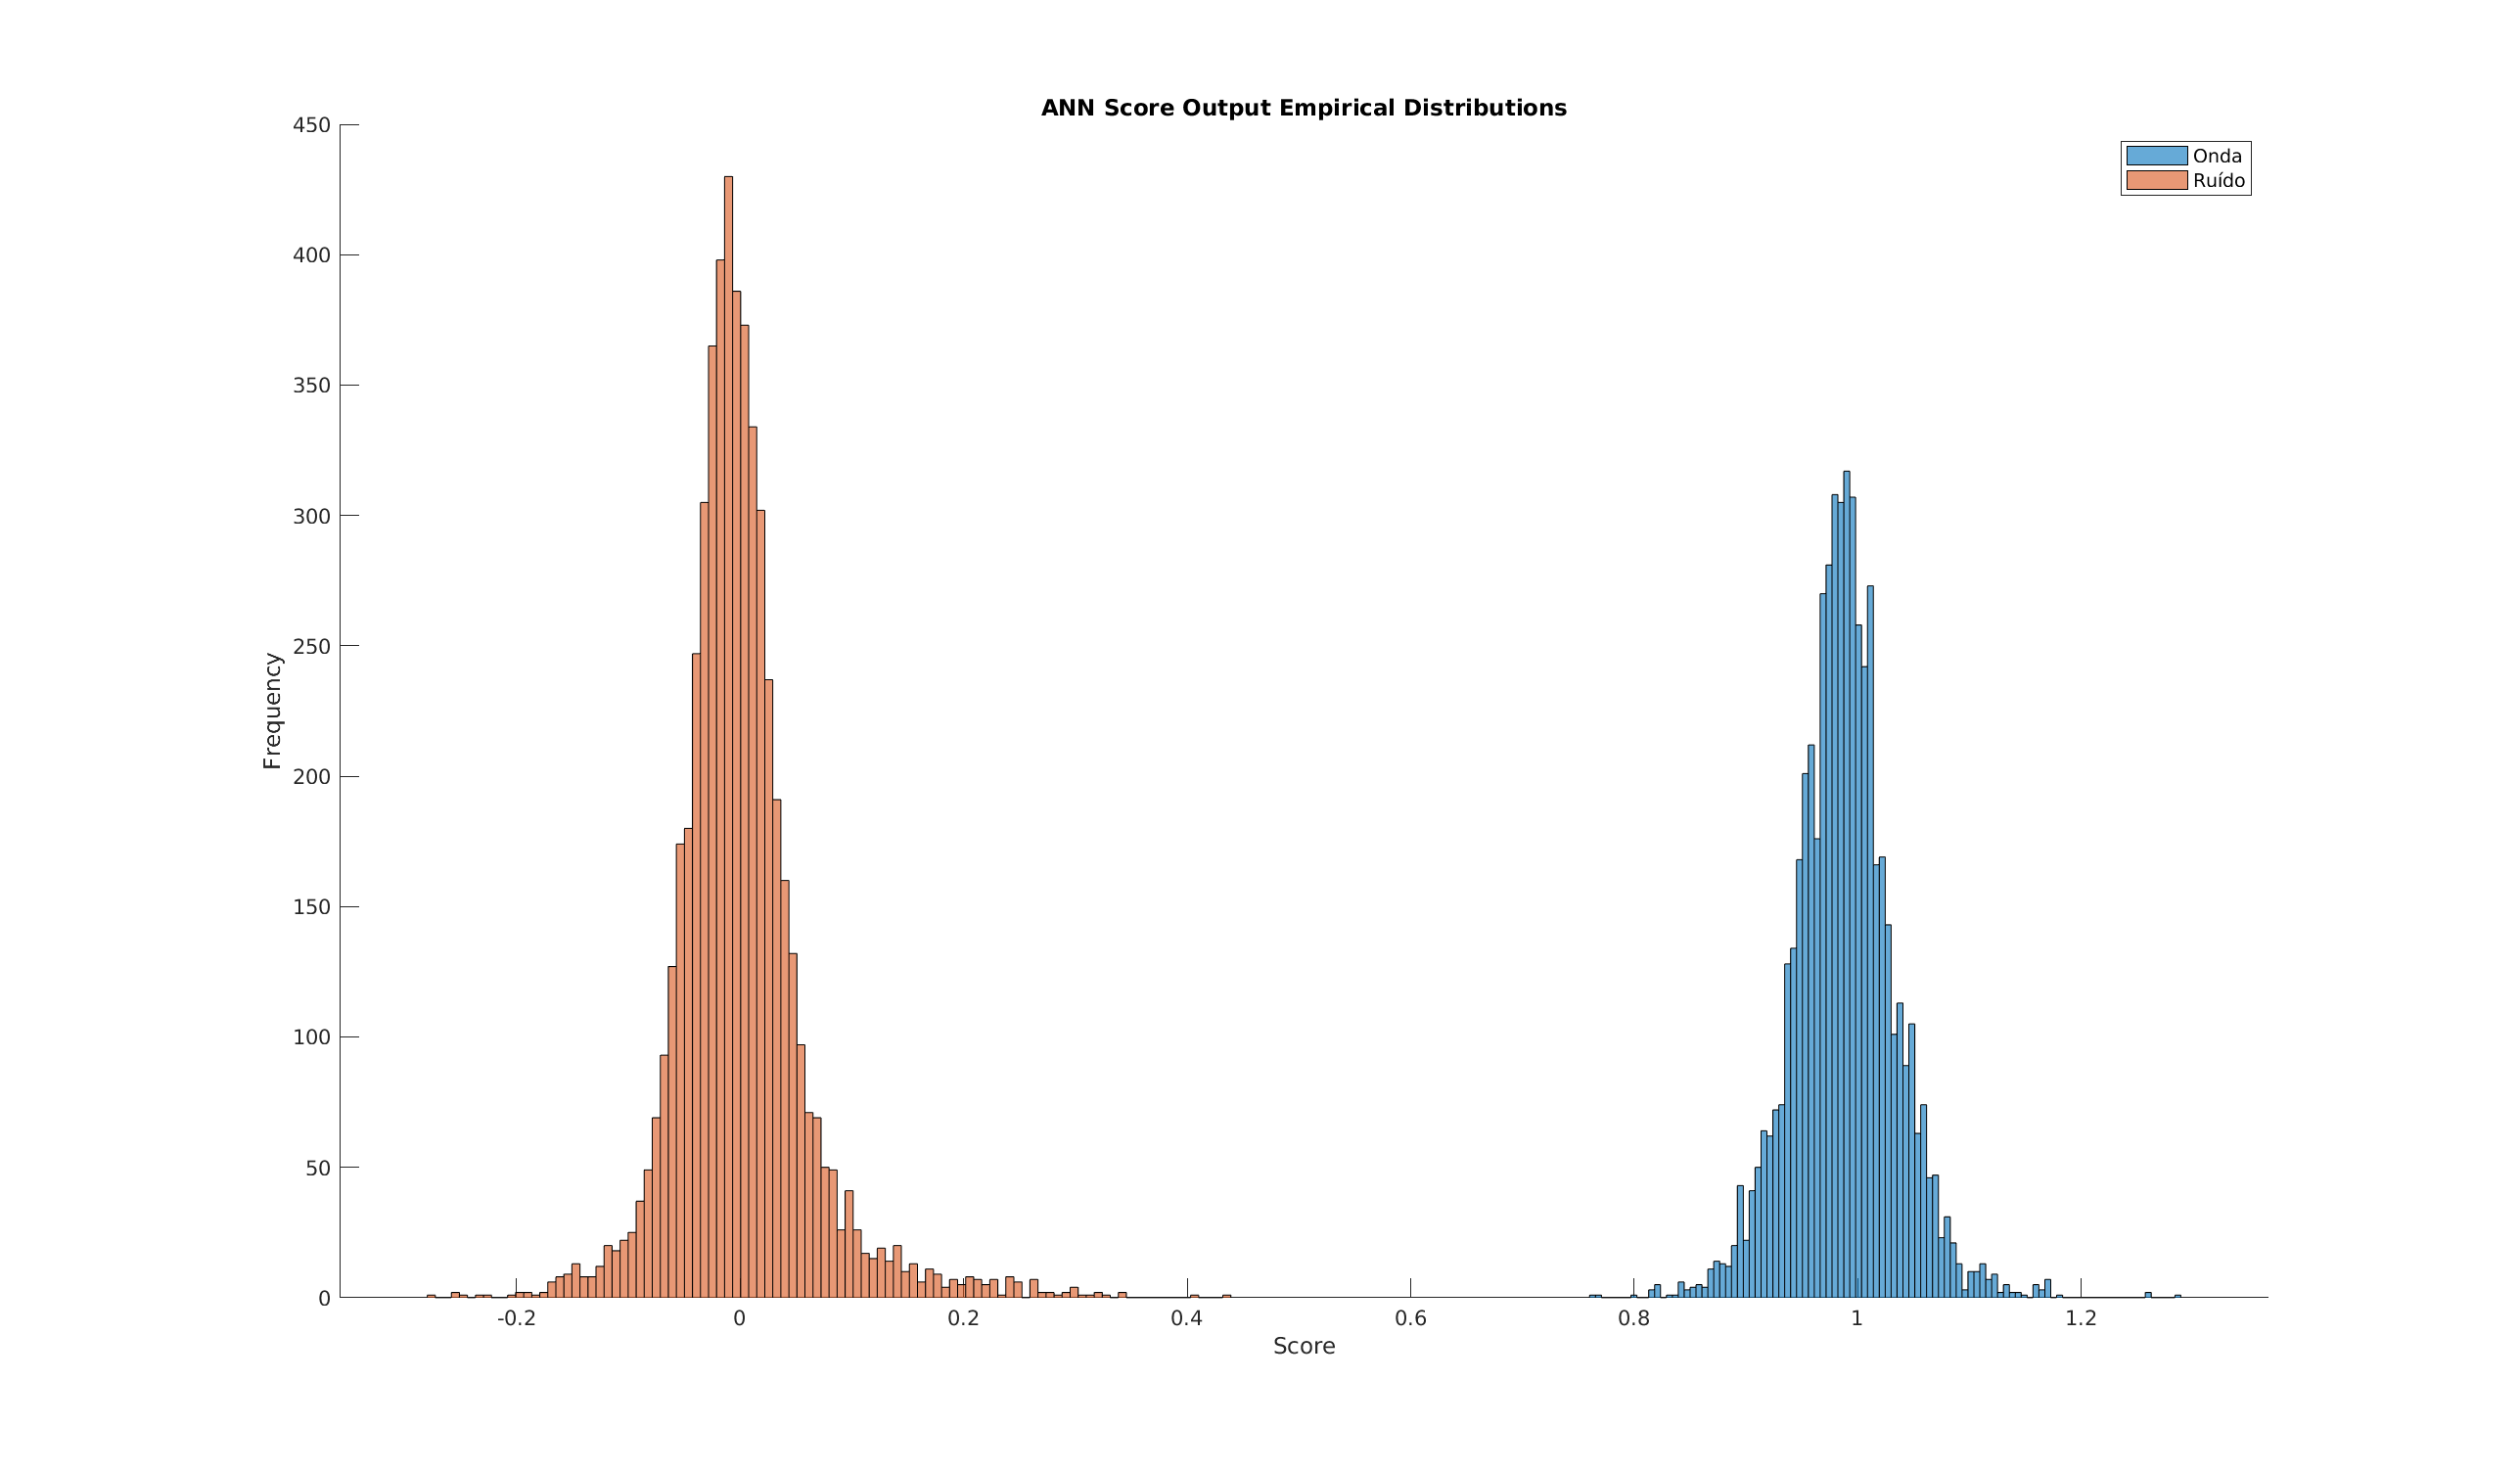
\includegraphics[width=1\textwidth]{figuras/histograma.eps}
\caption{Score da RNA para as duas classes (Onda e Ruído) - Distribuição empírica do score.}
\label{fig:histograma}
\end{figure}

A Figura~\ref{fig:KS} apresenta a distância KS entre essas duas distribuições. É notável ver a separação das duas classes, pois, as distribuições não tem ponto de intersecção em comum. Portanto, o modelo distingue perfeitamente o que é um Onda Gravitacional tanto quanto o que é Ruído. Como a separação das duas distribuições foi muito evidente, o valor do KS assume o valor máximo de 1.

\begin{figure}[H]
\centering
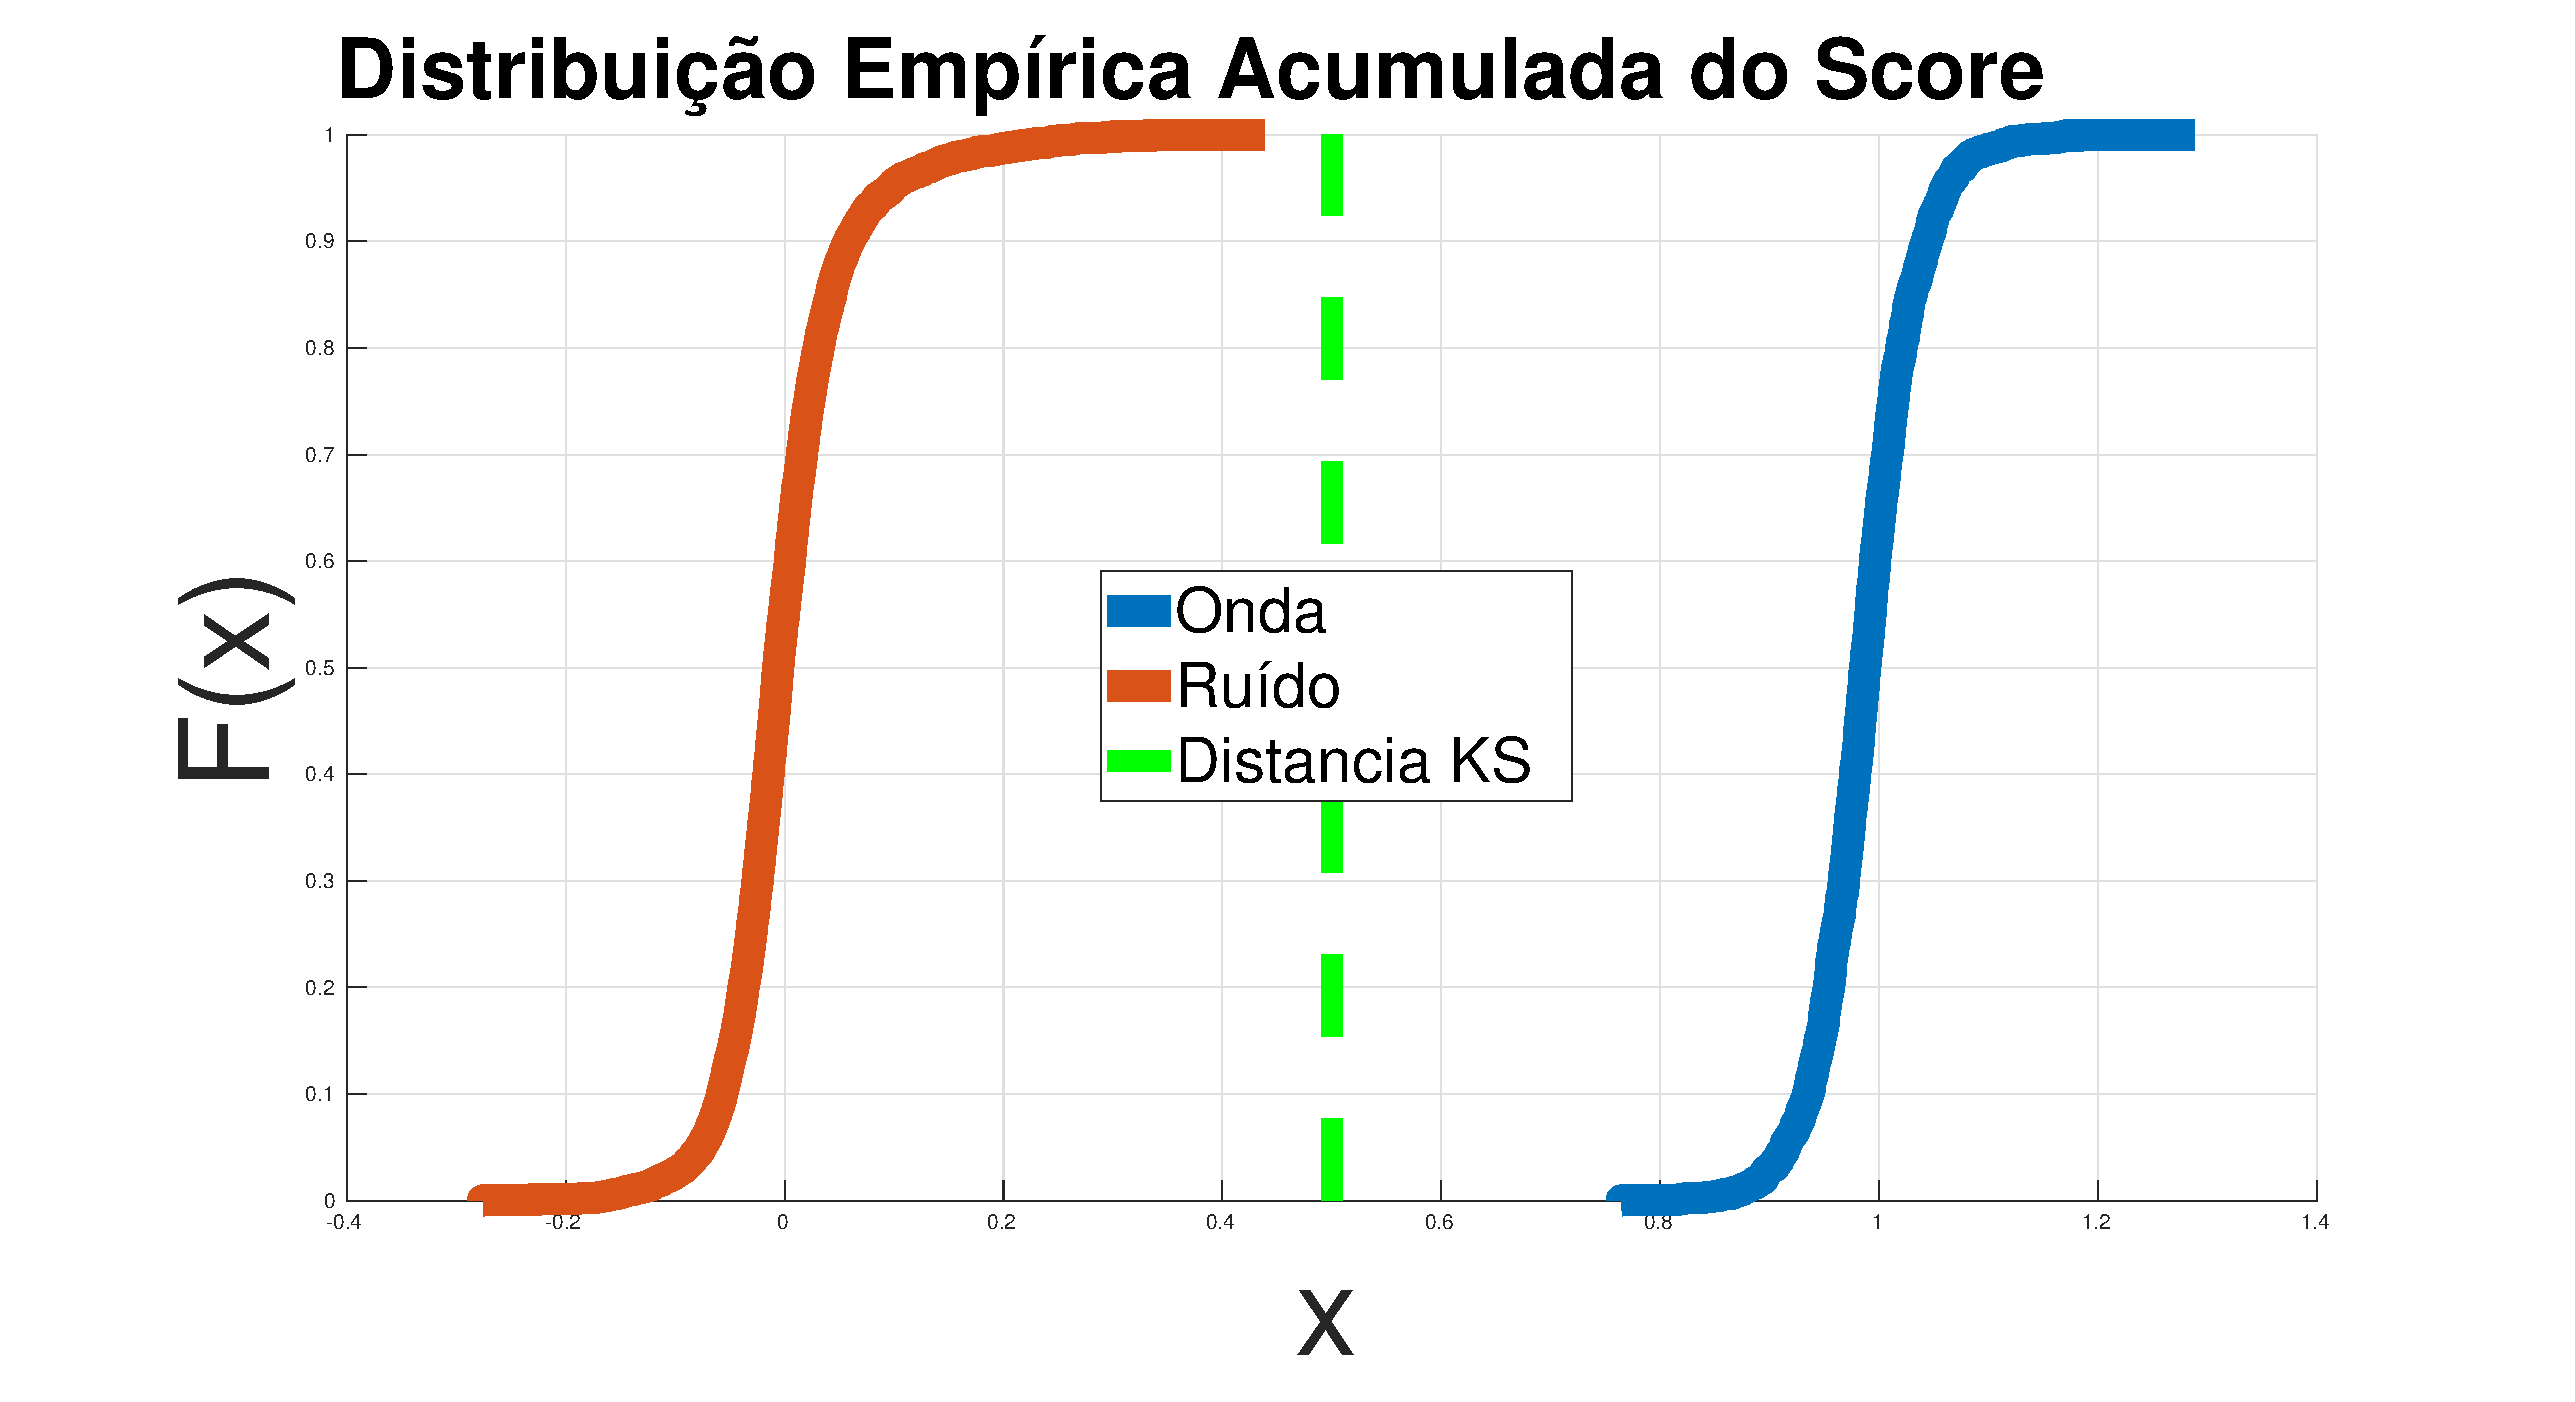
\includegraphics[width=1\textwidth]{figuras/KS.eps}
\caption{Score da RNA para as duas classes (Onda e Ruído) - Distribuição acumulada empírica do score.}
\label{fig:KS}
\end{figure}

Logo após encontrar o melhor modelo o comitê de RNA foi formado com as 500 melhores redes conforme mostra a Figura~\ref{fig:comite}. O critério de seleção das RNAs para o comitê, deu-se somente pelo MSE, dado que, todas as rede com a configuração descrita acima apresentam uma discriminação excelente como foi comprovado pelas Figuras~\ref{fig:histograma} e~\ref{fig:KS}.

Depois disso, quando o comitê recebeu os dados reais do LIGO para análise, um valor de score foi gerado. Foi gerado um score para cada um dos observatórios (H1 e L1) do LIGO para cada uma das nove ondas selecionadas.

Existem duas formas de analisar esse valor do score. Na primeira metodologia, na fase de treinamento, é determinado um valor de pontuação limite, em que valores inferiores a esse limite serão classificados como classe "Ruído" e valores maiores que esse limite serão classificados como classe "Onda". 

A segunda metodologia é considerar a distribuição empírica do score como uma função de pertinência (Lógica Fuzzy). Assim, o valor do score pode ser visto como um termômetro, onde valores baixos do score implicam na classe "Ruído" e valores altos do score na classe "Onda".

Neste sentido esta pesquisa adotou a segunda metodologia a qual trata o score como um termômetro de ondas gravitacionais. Portanto o conjunto criado de dados reais do LIGO e separados em janelas deslizantes, produz resultados de um score ao longo do tempo, a medida que a janela deslizante percorre os dados.

A Figura~\ref{fig:detection} mostra este resultado após a rede ser submetida aos dados da onda gravitacional GW150914 do laboratório Hanford(H1). Nesta imagem é possível notar o valor do score ao longo do tempo, em que, em certo ponto o score cresce a medida que a janela deslizante apresenta a onda gravitacional ao classificador, até o ponto em que o score atinge o valor 1, onde a janela deslizante esta centrada na onda gravitacional. Por outro lado, quando a janela deslizante avança e a onda gravitacional sai do foco e é finalizada o score volta a se aproximar de zero e permanece próximo até o final da classificação.

\begin{figure}[H]
\centering
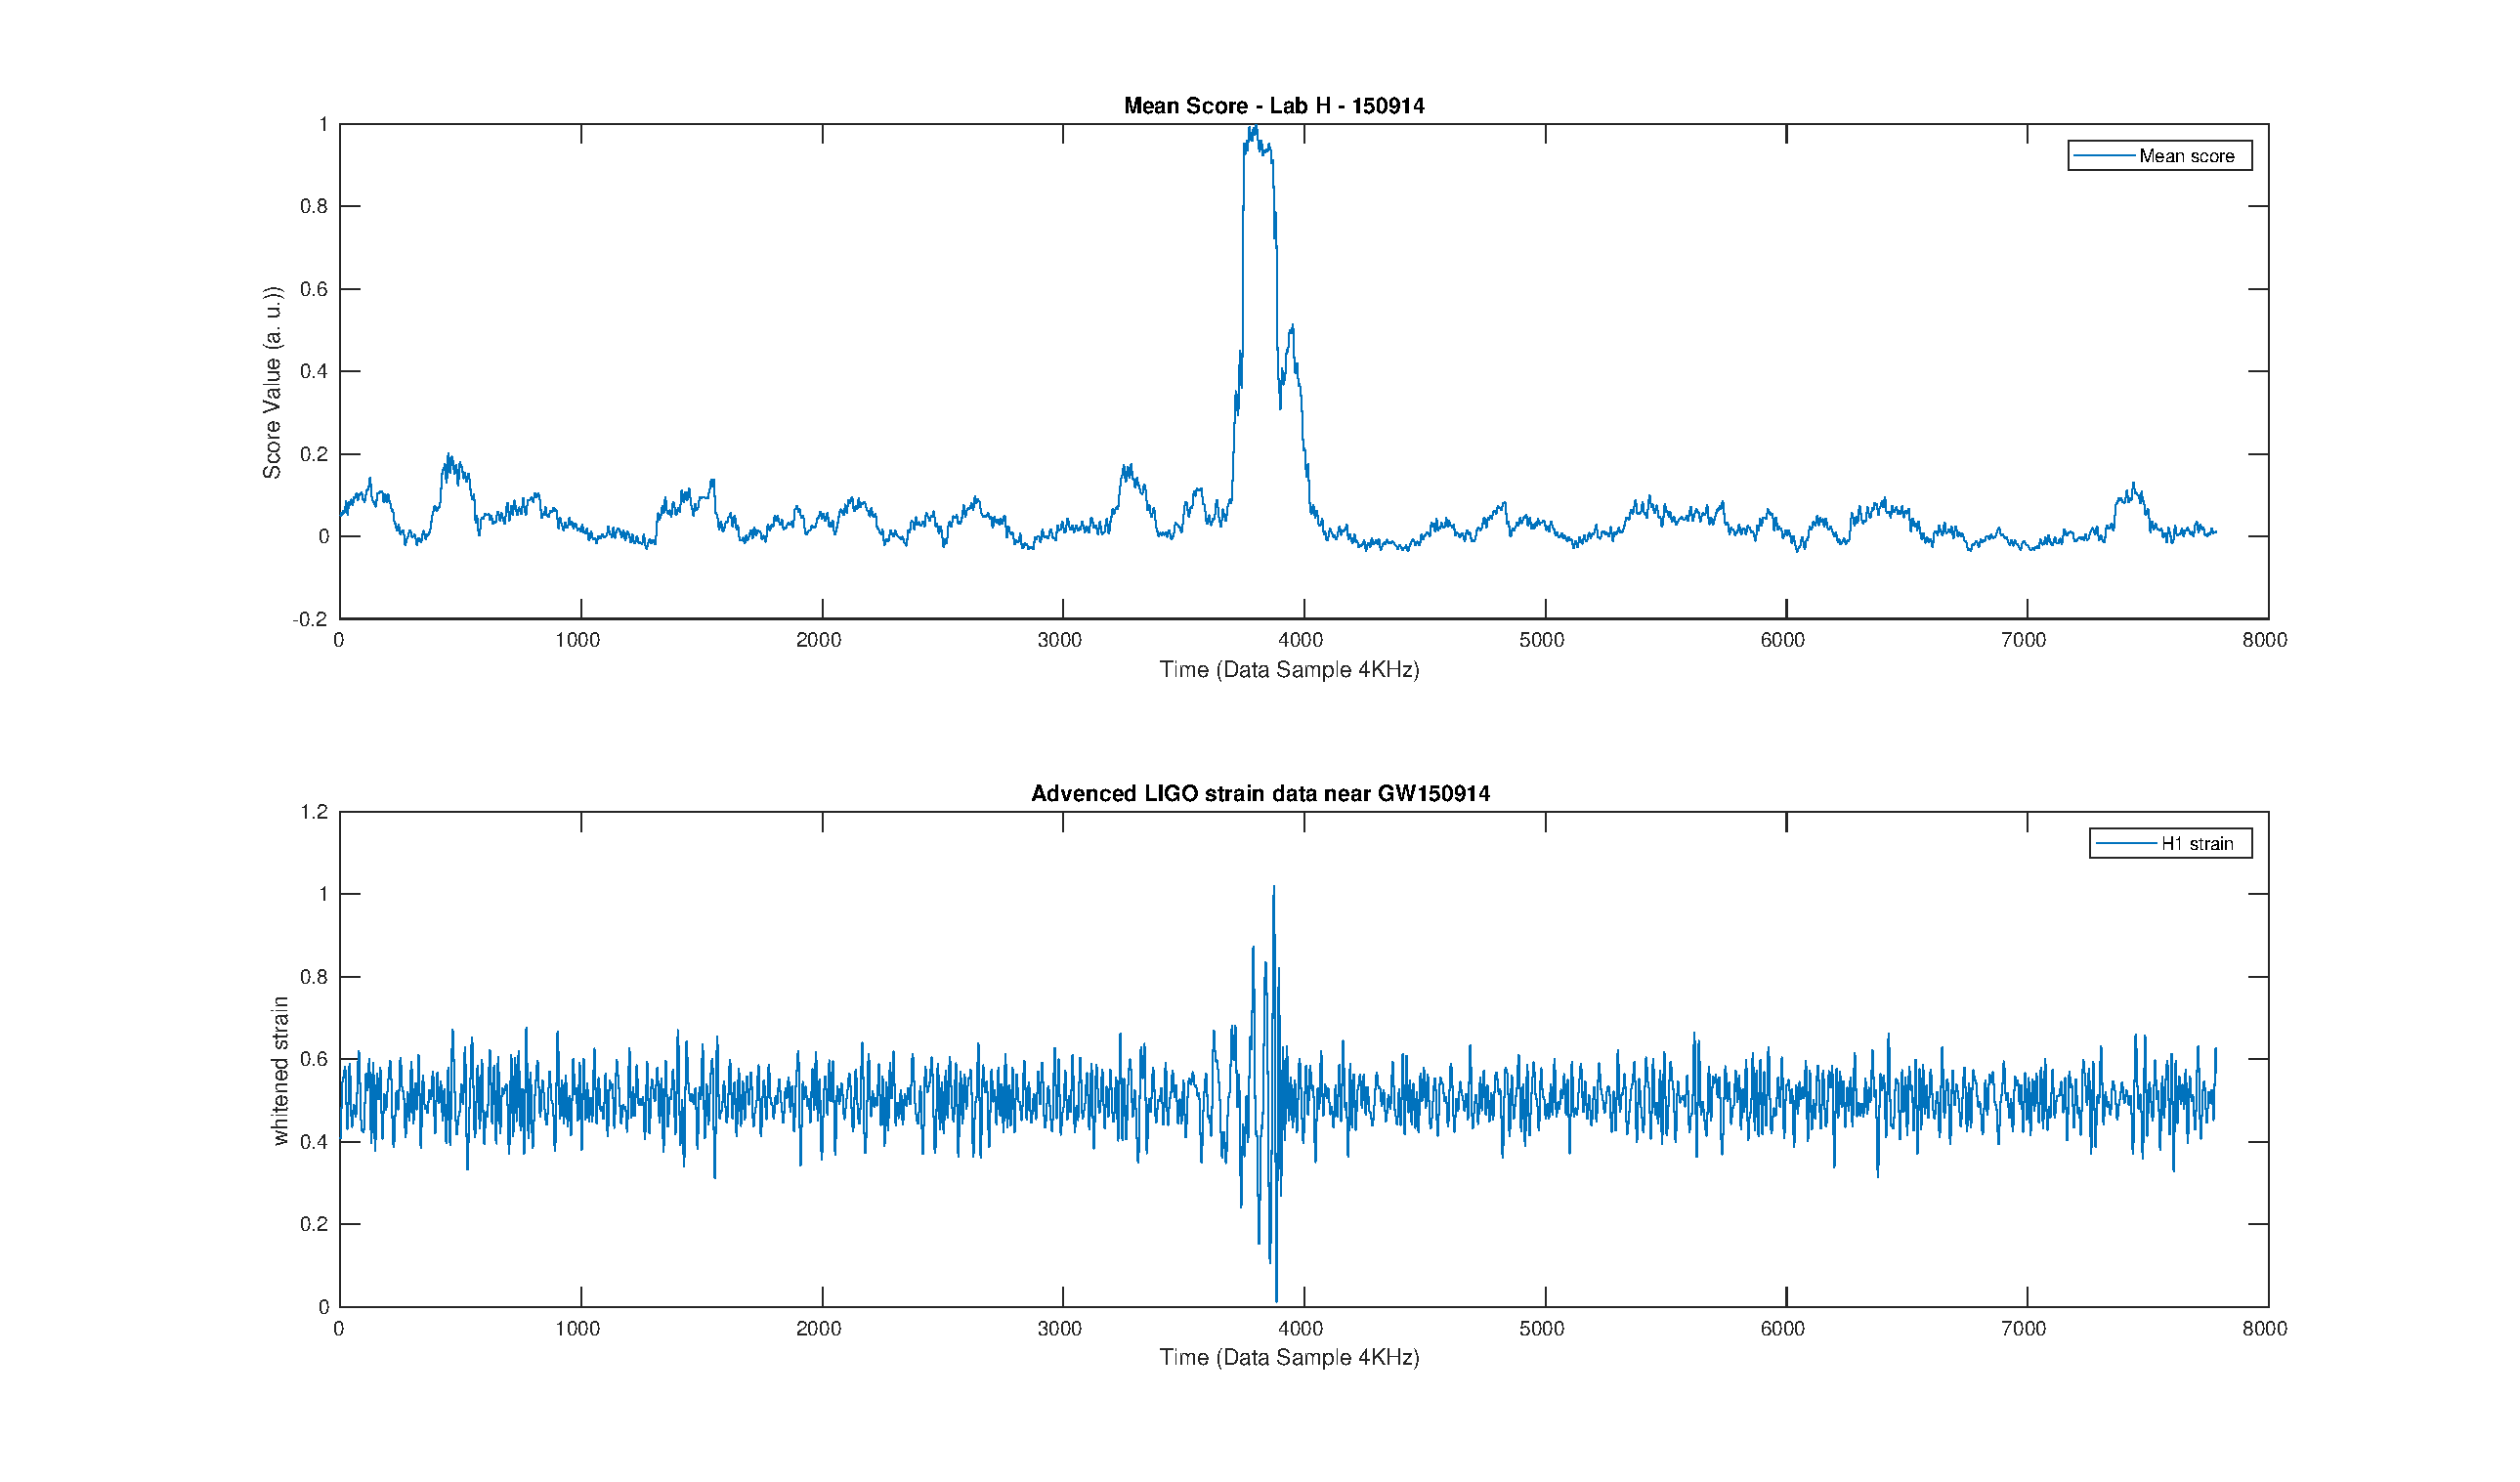
\includegraphics[width=1\textwidth]{figuras/detection.eps}
\caption{Resultado do score do comitê em comparação com os dados de entrada}
\label{fig:detection}
\end{figure}

Assim como o LIGO faz para confirmar a detecção das GW, esta pesquisa adotou a mesma premissa e usou os scores gerados para os dois laboratórios do LIGO, Figura~\ref{fig:score-H1} e~\ref{fig:score-L1} para fazer uma coincidência entre os dados, afim de confirmar a detecção da onda gravitacional.

\begin{figure}[H]
     \centering
     \begin{subfigure}[b]{0.45\textwidth}
         \centering
         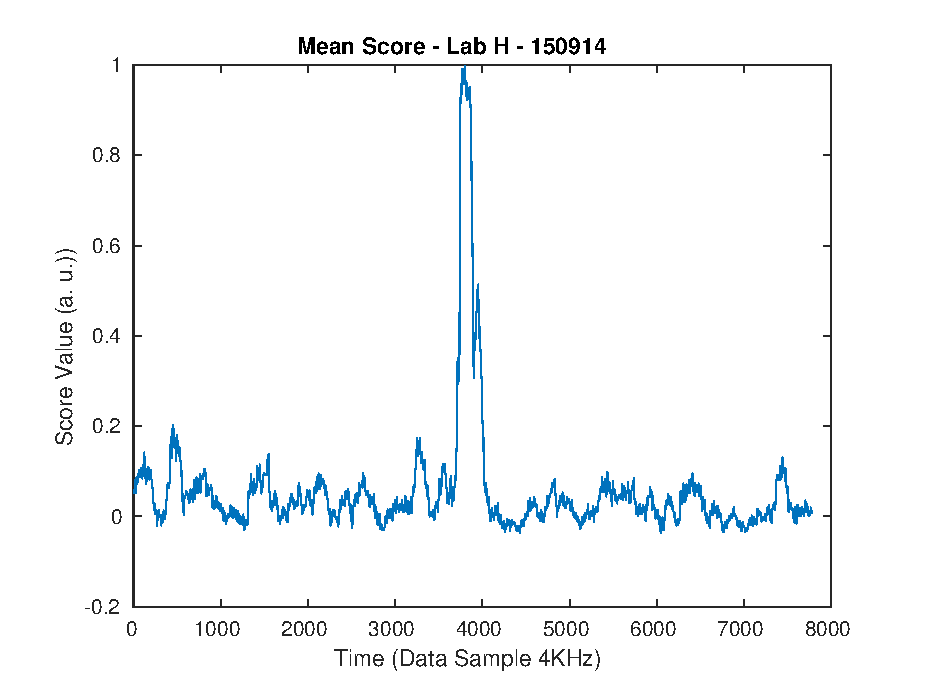
\includegraphics[width=\textwidth]{figuras/GW150914_LabH.eps}
         \caption{Score gerado para o laboratório H}
         \label{fig:score-H1}
     \end{subfigure}
     \hfill
     \begin{subfigure}[b]{0.45\textwidth}
         \centering
         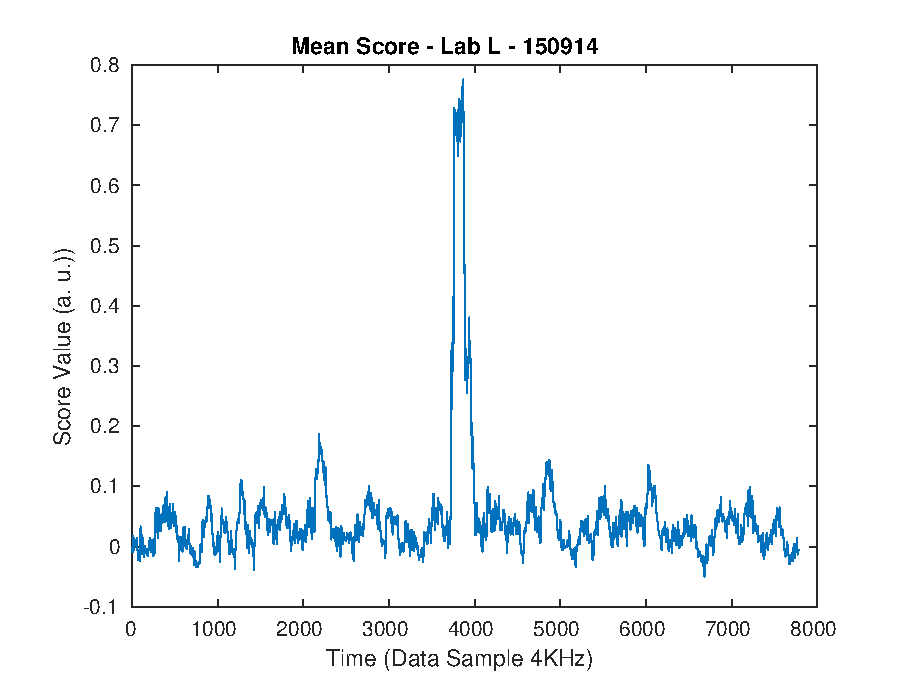
\includegraphics[width=\textwidth]{figuras/GW150914_LabL.eps}
         \caption{Score gerado para o laboratório L}
         \label{fig:score-L1}
     \end{subfigure}
     \caption{Score da onda gravitacional GW150914}
\end{figure}

O resultado desta coincidência de dados gerou um novo score muito mais limpo e claro sobre a detecção da onda gravitacional. Na Figura~\ref{fig:scoreHL} é mostrado o resultado da coincidência entre os scores da GW150914 gerados para os dois laboratórios do LIGO.

\begin{figure}[H]
\centering
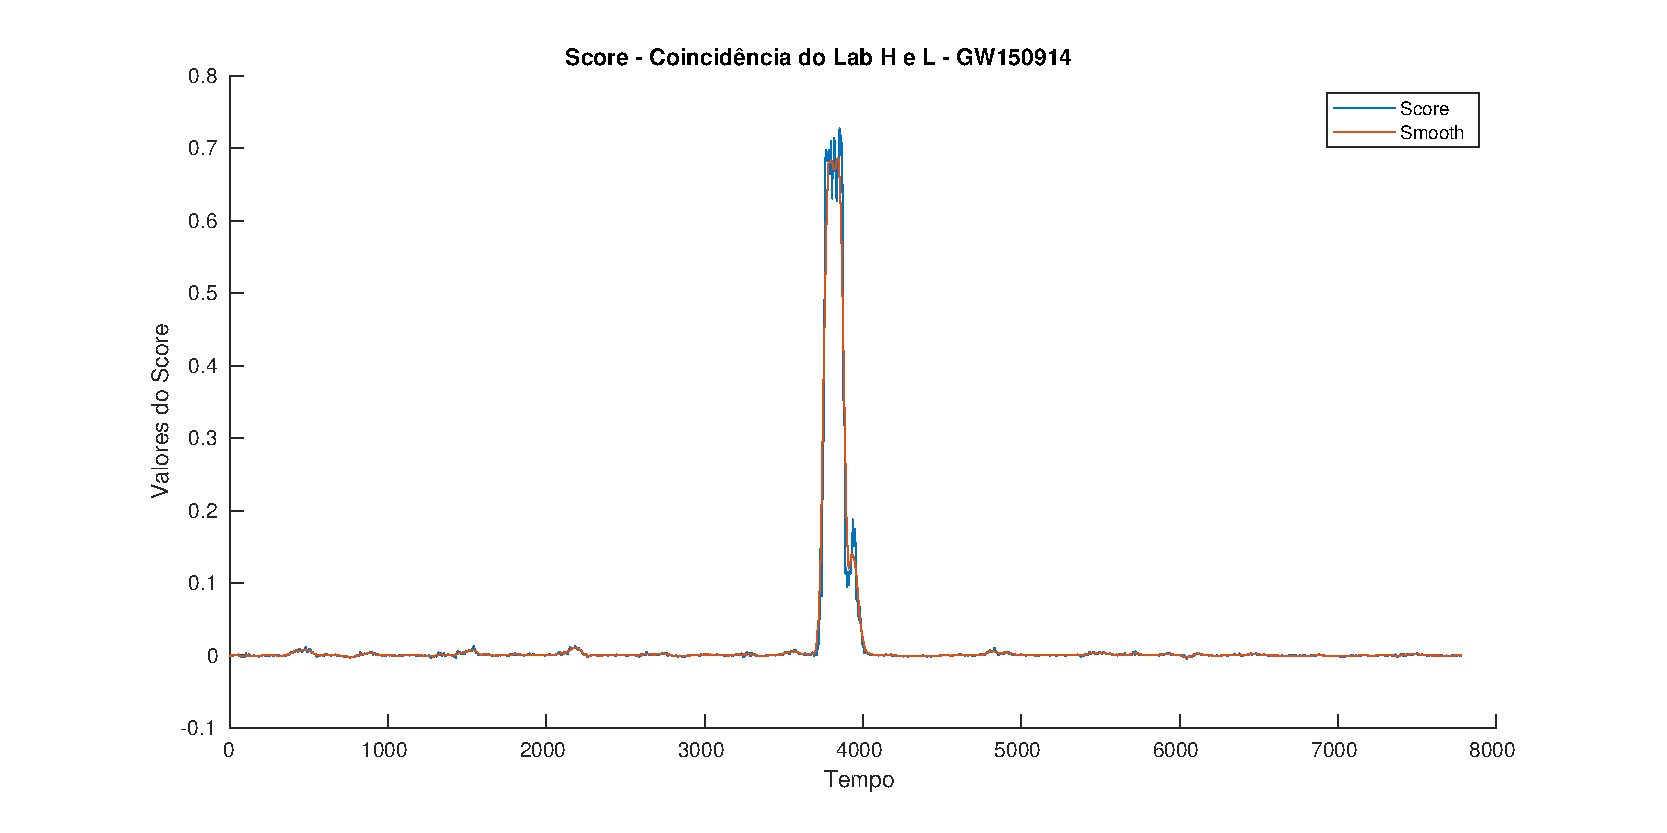
\includegraphics[width=1\textwidth]{figuras/GW150914_LabHL.eps}
\caption{Resultado do score da RNA em comparação com os dados reais do LIGO.}
\label{fig:scoreHL}
\end{figure}

Para uma melhor visualização dos resultados na Figura~\ref{fig:scoreHL} é possível notar que foi feito uma suavização dos dados, representada pela linha vermelha (Smooth). Nesta Figura~\ref{fig:scoreHL} diferente dos resultados individuais de cada laboratório do LIGO, não alcança a margem do valor máximo de 1, pois apos a coincidência dos dados entre os laboratórios, este valor tende a ficar menos, mas a sua representação esta mais que clara que demostra a detecção da onda gravitacional em meio aos dados. A Figura~\ref{fig:scoreHLZoom} mostra um zoom deste resultado.

\begin{figure}[H]
\centering
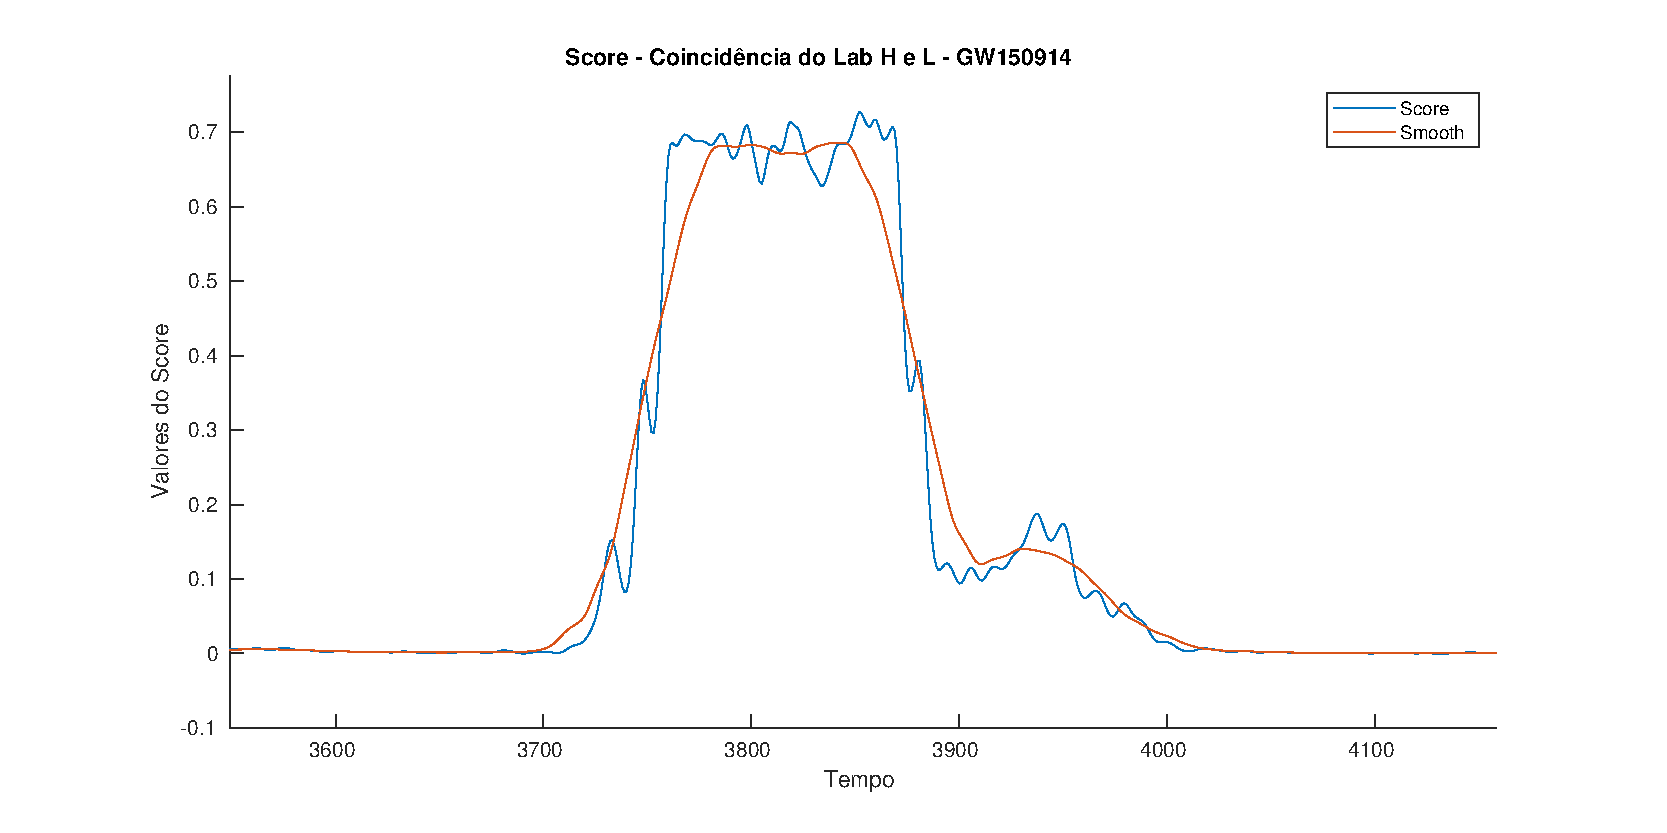
\includegraphics[width=1\textwidth]{figuras/GW150914_LabHL_zoom.eps}
\caption{Zoom do resultado da coincidência entre os laboratórios H1 e L1 para a GW150914.}
\label{fig:scoreHLZoom}
\end{figure}

É possível ver todos os resultados obtidos nesta pesquisa no Apendice A.